% Options for packages loaded elsewhere
\PassOptionsToPackage{unicode}{hyperref}
\PassOptionsToPackage{hyphens}{url}
%
\documentclass[
]{scrartcl}
\usepackage{amsmath,amssymb}
\usepackage{lmodern}
\usepackage{iftex}
\ifPDFTeX
  \usepackage[T1]{fontenc}
  \usepackage[utf8]{inputenc}
  \usepackage{textcomp} % provide euro and other symbols
\else % if luatex or xetex
  \usepackage{unicode-math}
  \defaultfontfeatures{Scale=MatchLowercase}
  \defaultfontfeatures[\rmfamily]{Ligatures=TeX,Scale=1}
\fi
% Use upquote if available, for straight quotes in verbatim environments
\IfFileExists{upquote.sty}{\usepackage{upquote}}{}
\IfFileExists{microtype.sty}{% use microtype if available
  \usepackage[]{microtype}
  \UseMicrotypeSet[protrusion]{basicmath} % disable protrusion for tt fonts
}{}
\makeatletter
\@ifundefined{KOMAClassName}{% if non-KOMA class
  \IfFileExists{parskip.sty}{%
    \usepackage{parskip}
  }{% else
    \setlength{\parindent}{0pt}
    \setlength{\parskip}{6pt plus 2pt minus 1pt}}
}{% if KOMA class
  \KOMAoptions{parskip=half}}
\makeatother
\usepackage{xcolor}
\IfFileExists{xurl.sty}{\usepackage{xurl}}{} % add URL line breaks if available
\IfFileExists{bookmark.sty}{\usepackage{bookmark}}{\usepackage{hyperref}}
\hypersetup{
  pdftitle={Topological Aspects of Symmetry in Low Dimensions},
  pdfauthor={Kantaro Ohmori,  University of Tokyo},
  hidelinks,
  pdfcreator={LaTeX via pandoc}}
\urlstyle{same} % disable monospaced font for URLs
\usepackage{longtable,booktabs,array}
\usepackage{calc} % for calculating minipage widths
% Correct order of tables after \paragraph or \subparagraph
\usepackage{etoolbox}
\makeatletter
\patchcmd\longtable{\par}{\if@noskipsec\mbox{}\fi\par}{}{}
\makeatother
% Allow footnotes in longtable head/foot
\IfFileExists{footnotehyper.sty}{\usepackage{footnotehyper}}{\usepackage{footnote}}
\makesavenoteenv{longtable}
\usepackage{graphicx}
\makeatletter
\def\maxwidth{\ifdim\Gin@nat@width>\linewidth\linewidth\else\Gin@nat@width\fi}
\def\maxheight{\ifdim\Gin@nat@height>\textheight\textheight\else\Gin@nat@height\fi}
\makeatother
% Scale images if necessary, so that they will not overflow the page
% margins by default, and it is still possible to overwrite the defaults
% using explicit options in \includegraphics[width, height, ...]{}
\setkeys{Gin}{width=\maxwidth,height=\maxheight,keepaspectratio}
% Set default figure placement to htbp
\makeatletter
\def\fps@figure{htbp}
\makeatother
\setlength{\emergencystretch}{3em} % prevent overfull lines
\providecommand{\tightlist}{%
  \setlength{\itemsep}{0pt}\setlength{\parskip}{0pt}}
\setcounter{secnumdepth}{5}
\usepackage{braket}
\numberwithin{equation}{section}
\ifLuaTeX
  \usepackage{selnolig}  % disable illegal ligatures
\fi
\usepackage[sorting=none]{biblatex}
\addbibresource{ref.bib}

\title{Topological Aspects of Symmetry in Low Dimensions}
\author{Kantaro Ohmori, University of Tokyo}
\date{2022-02-13}

\usepackage{amsthm}
\newtheorem{theorem}{Theorem}[section]
\newtheorem{lemma}{Lemma}[section]
\newtheorem{corollary}{Corollary}[section]
\newtheorem{proposition}{Proposition}[section]
\newtheorem{conjecture}{Conjecture}[section]
\theoremstyle{definition}
\newtheorem{definition}{Definition}[section]
\theoremstyle{definition}
\newtheorem{example}{Example}[section]
\theoremstyle{definition}
\newtheorem{exercise}{Exercise}[section]
\theoremstyle{definition}
\newtheorem{hypothesis}{Hypothesis}[section]
\theoremstyle{remark}
\newtheorem*{remark}{Remark}
\newtheorem*{solution}{Solution}
\begin{document}
\maketitle
\begin{abstract}
This is a lecture note prepared for ``26th APCTP Winter School on Fundamental Physics'', Feb.~14-18, 2022.

In this lecture we will study the symmetry and its anomaly in low-dimensional, i.e.~0+1d and 1+1d, quantum field theories.
In 0+1-dimensional quantum field theory, a.k.a quantum mechanics, the Wigner's theorem tells that a global symmetry forms a group and acts on the Hilbert (state) space as a projective representation. We will see example with non-trivial projective phases and how it can be related to symmetry protected topological phases in 1+1-dimensions. We then see how the story are generalized/changed in 1+1-dimensional (relativistic) quantum field theory, where the locality of the theory plays an important role.
Time permits, we also see how the inclusion of fermions affects the story.
\end{abstract}

{
\setcounter{tocdepth}{2}
\tableofcontents
}
\hypertarget{introduction}{%
\section{Introduction}\label{introduction}}

Symmetry is a guiding principle in physics. In many case, given a system, you first analyze its symmetry. Or, to model a given phenomena, the symmetry is often be the first clue.
Therefore, there have been numerous research on the topic. What is surprising is that, still, in 2022, it is a hot area of research and there are many things to be understood.

\hypertarget{lecture-guide}{%
\subsection{Lecture guide}\label{lecture-guide}}

\hypertarget{usage-of-this-note}{%
\subsubsection{Usage of this note}\label{usage-of-this-note}}

This note is provided primarily as a website.
The usage is self-explaining but you might find a useful tips if you click the ``i'' mark in the top navigation bar. Also from the navigation bar one can download the pdf version. (If you want a epub file, I can easily generate it too, so let me know.) \textbf{However, the equation number does not much currently between the html and pdf format.}

The parts having * at the tail of its title will probably be skipped in the lecture.

\hypertarget{objective}{%
\subsubsection{Objective}\label{objective}}

This lecture aims to be an introduction to the field of symmetry and its anomaly in quantum field theory (QFT). In the first part of the lecture topological aspects of symmetry in quantum mechanics are reviewed, then in the latter part of the lecture we proceed to symmetry in 1+1-dimensional quantum field theory.

\hypertarget{prerequisite}{%
\subsubsection{Prerequisite}\label{prerequisite}}

Proficiency in the undergraduate level quantum mechanics and some basic knowledge about quantum field theory and group theory (e.g.~what are \(SO(3)\), \(SU(2)\), \(\mathbb{Z}_2\), and so on) are assumed, but (hopefully) not much more. Especially, the first half will focus on quantum mechanics so it is hopefully understandable to even advanced undergraduates.

\hypertarget{useful-references}{%
\subsubsection{Useful references}\label{useful-references}}

\begin{enumerate}
\def\labelenumi{\arabic{enumi}.}
\tightlist
\item
  \textcite{tachikawa_2019}:
  The first half of Yuji's lecture is about the big framework the most of researchers assume (but not necessarily proven), which I will omit.
  The second half of Yuji's will serve as an advanced version of this lecture.
\item
  \textcite{Witten:2015aoa}, \textcite{Witten:2015aba}:
  While there are not so much overlap between this lecture by me and these lecture note and paper by E. Witten, and Witten's is a bit more advanced, they are undoubtedly ones of the best entry points to the field.
\end{enumerate}

\hypertarget{motivation}{%
\subsection{Motivation}\label{motivation}}

Why do we care about symmetry and its anomaly in quantum field theory?
There are two (closely related) uses cases of symmetry and its anomaly in the study of QFT and its applications:

\begin{enumerate}
\def\labelenumi{\arabic{enumi}.}
\tightlist
\item
  to construction of a model, given observed spectrum or other desired properties, and
\item
  to constraining possible long range physics from 't Hooft anomaly matching.
\end{enumerate}

An example for the case one is the Standard Model (SM) of the particle physics.
The spectrum of the fermions fits into a representation of \(SU(3)\times SU(2) \times U(1)\) nicely, and gauging of the symmetry, after including the Higgs boson, magically explains almost all physics that occur in a collider. (The finding of the quark model involving the color symmetry was also mainly from group theory: it was to reproduce the observed \(SU(3)\) symmetry among hadrons. )

The quantum anomaly is also very important in construction of the SM: a single family of fermions in SM has chiral spectrum but seemingly miraculous cancellation of the quantum anomaly, which makes the model consistent. This cancellation also leads to the idea of grand unification.

The second case is about the quantum anomaly for \emph{global} symmetry.\footnote{Some authors, including the author of this lecture note, sometimes use the term ``'t Hooft anomaly'', to mean a quantum anomaly for a \emph{global} symmetry, to distinguish it from a quantum anomaly involving \emph{gauge} symmetry. However this terminology does not seem to have a historical root (while the term ``'t Hooft anomaly matching'' is easily justified), so in this lecture KO tries to avoid the terminology to avoid any possible confusion.}
't Hooft anomaly matching states that the anomaly should match between the UV and IR of an renormalization group (RG) flow (see Fig. \ref{fig:flow}).
Let \(G_\text{UV}\) and \(G_\text{IR}\) be the symmetry group for the UV and IR theory, respectively.
The existence of the RG flow between them in particular means that an isomorphism between them:
\begin{equation}
  \label{eq:Ghom}
  \phi: G_\text{UV} \to G_\text{IR}.
\end{equation}
The RG flow also assigns a map between the quantum anomalies, which are a property of symmetries in a local quantum system, for the symmetries \(G_\text{UV}\) and \(G_\text{IR}\);
but this time it is backwards:
\begin{equation}
  \label{eq:pullback}
  \phi^*: \mathcal{A}_\text{IR} \to \mathcal{A}_\text{UV}.
\end{equation}
This map is in a sense linear, in particular \(\phi^* (0) = 0\), where \(\mathcal{A}=0\) means that there is no anomaly.
Therefore, if you know that \(\mathcal{A}_\text{UV}\neq 0\), which immediately means \(\mathcal{A}_\text{IR}\neq 0\).
In turn, you also conclude that the IR \emph{theory} it self is \emph{not} trivial: you need some degrees of freedom to \textbf{match} the anomaly.

This is the power of 't Hooft anomaly matching: that you can say something without analyzing the dynamics about where the theory can flow into.
This can be done even if the theory is very hard to analyze, i.e.~\emph{strongly coupled}, for example asymptotically free theories.
For such theories the anomaly matching (and some generalization) are sometimes the only, or one of the few, analytical tools that one can apply.
Thus the 't Hooft anomaly matching is a part of the foundation in the research of strongly coupled quantum systems.

\begin{figure}

{\centering 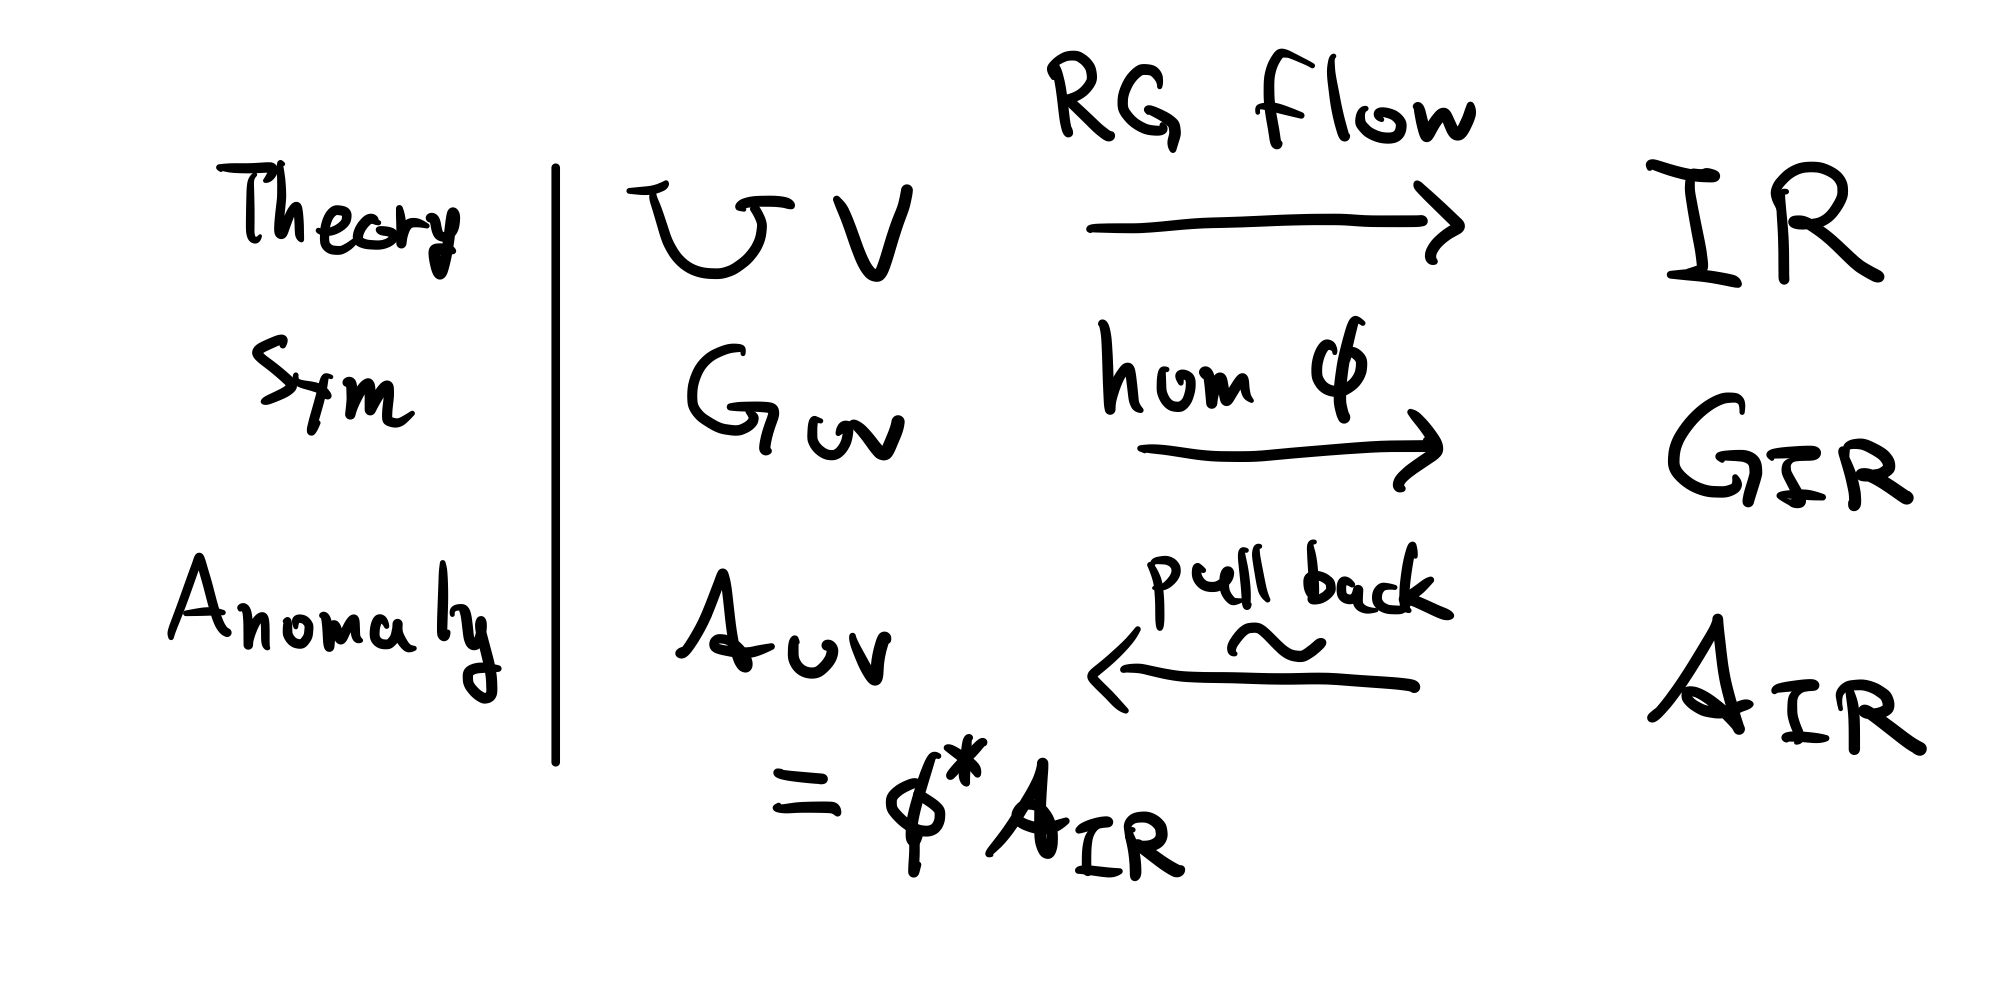
\includegraphics[width=0.5\linewidth]{figs/flow_symmetry} 

}

\caption{'t Hooft anomaly matching}\label{fig:flow}
\end{figure}

\hypertarget{quantum-anomaly-in-quantum-mechanics}{%
\section{Quantum Anomaly in Quantum Mechanics}\label{quantum-anomaly-in-quantum-mechanics}}

In this chapter we learn about quantum anomaly of a symmetry in quantum mechanics, without assuming any kind of locality.
Here, locality roughly means that we have a notion of ``observables localized in a subregion of the space (or spacetime).''
Both quantum field theory (QFT) and a quantum system on lattice are local in this sense, which greatly affect the possible behavior of a symmetry.
Here we will see what kind of ``topological'' phenomena are possible regarding symmetry when the locality is absent.
In such case, we often regard that all of the observables are associated to a single point consisting the entire ``space'', justifying call such a system ``0+1-dimensional.''

\hypertarget{basics-about-quantum-mechanics}{%
\subsection{Basics about quantum mechanics}\label{basics-about-quantum-mechanics}}

Let us recall the basics.
Given a quantum system, we have a Hilbert space \(\mathcal{H}\),
in which a state lives.
A unit state \(\ket{\psi}\) and another \(\ket{\psi'}\) describes the same state, which we write as \(\ket{\psi}\sim\ket{\psi'}\), if (and only if)
\begin{equation}
  \label{eq:phase-equiv}
  \ket{\psi} = e^{\mathrm{i}\alpha}\ket{\psi'}
\end{equation}
for some phase \(\alpha\).
Then, we define the \emph{ray space} \(\mathbb{P}\mathcal{H}\) as the projective space of \(\mathcal{H}\):
\begin{equation}
  \label{eq:PH}
  \mathbb{P}\mathcal{H} := S\mathcal{H}/\sim,
\end{equation}
where \(S\mathcal{H}\) denotes the space of unit states.
By definition, elements in the ray space are one-to-one corresponded to physical states of the system.
Given two states \([\ket{\psi}],[\ket{\phi}] \in \mathbb{P}\mathcal{H}\), where \([,]\) denotes the equivalence class in the definition \eqref{eq:PH}, the transition probability of the two states are
\begin{equation}
  \label{eq:transprob}
  \lvert \braket{\psi|\phi}\rvert^2.
\end{equation}
Note that this definition does not depends on the choice of the representatives \(\psi,\phi\) in each class.
We put the structure of abelian group to \(C^2(G,M)\) induced by the abelian group structure of \(M\).

Sometimes it is convenient to focus on \emph{operators} acting on the states, rather than the states itself.
We let the algebra of the (bounded) operators be denoted by \(\mathcal{A}\).
If the Hilbert space is finite dimensional, i.e.~\(\mathcal{H} = \mathbb{C}^n\) for some integer \(n\),
the algebra is simply the matrix algebra:
\begin{equation}
  \label{eq:Amatrix}
  \mathcal{A} \cong \mathrm{Mat}(\mathbb{C}^n).
\end{equation}

In this lecture we consider the dynamics by a constant Hamiltonian\footnote{Instead, one might consider a discrete (finite time) evolution by a unitary operator.
  Such a system is often called Floquet system. The term originally means that you have an external field periodic in the time. The discrepancy between the continuous and discrete evolutions is an interesting ongoing research topic.}.
We use the Heisenberg picture, so the state \(\ket{\psi}\) does not develop but an operator \(\mathcal{O}\)
develops in time as
\begin{equation}
  \label{eq:Odev}
  \mathcal{O}(t) = e^{\mathrm{i}H t} \mathcal{O}(0) e^{-\mathrm{i}H t}.
\end{equation}
Here we have set the plank constant \(\hbar =1\).

\hypertarget{wigners-theorem}{%
\subsection{Wigner's theorem}\label{wigners-theorem}}

According to E. Wigner, a \textbf{symmetry transformation} \(U\) acting on a quantum system is a bijection
\begin{equation}
  \label{eq:sym}
  T: \mathbb{P}\mathcal{H} \to \mathbb{P}\mathcal{H},
\end{equation}
that preserves the transition probability \eqref{eq:transprob}.
We call a bijection \(U\) on \(\mathcal{H}\) is compatible with \(T\) if \(U\) induces the same action on \(\mathbb{P}\mathcal{H}\) as \(T\).

Then, Wigner's theorem states:

\begin{theorem}[Wigner 1931]
Given a symmetry transformation \(T\), there exists a bijection \(U_T\) on \(\mathcal{H}\) compatible with \(T\).
This \(U_T\) is either linear (over \(\mathbb{C}\)) and unitary, or anti-linear and anti-unitary. If \(\mathrm{dim}\mathcal{H}\ge 2\), this \(U\) is unique up to a overall phase redefinition \(U_T \mapsto e^{\mathrm{i}\alpha}U_T\). (When \(\mathrm{dim}\mathcal{H} = 1\), \(T\) is unique, and \(U_T\) can be taken either of unitary or anti-unitary one. Once the choice is fixed, it is up to the phase.)
\end{theorem}

This is why we usually care about unitary operator (like Pauli matrices).
The proof can be found somewhere, e.g. \textcite{Weinberg:1995mt}. We will see examples soon.

We also have an action of \(T\) on the algebra of operators \(\mathcal{A}\) through this theorem:
\begin{align}
  \label{eq:TonA}
  T \curvearrowright \mathcal{A}  & \to \mathcal{A}\\
  \mathcal{O} & \mapsto U_T \mathcal{O} U^\dagger_T.
\end{align}
Note that this action is independent of the phase freedom of \(U_T\) and thus uniquely defined.
\eqref{eq:Odev} is a special case of this.

Finally, we call a symmetry \(T\) is \textbf{preserved} by the Hamiltonian if
\begin{equation}
  \label{eq:UHcommute}
  [U_T,H] = 0.
\end{equation}

\hypertarget{Bloch}{%
\subsection{Bloch sphere and projective representation}\label{Bloch}}

Let us take a close look at the case of a qubit, i.e.~\(\mathcal{H} = \mathbb{C}^2\).
Pick a basis \(\ket{0}\) and \(\ket{1}\) and expand a unit state \(\ket{\psi}\) as
\begin{equation}
  \label{eq:psiexp}
  \ket{\psi} = \cos(\theta/2) \ket{0} + \sin(\theta/2)e^{\mathrm{i}\phi} \ket{1},
\end{equation}
where \(0\le \theta \le \pi\) and \(0 \le \phi \le 2\pi\).
One can always bring a unit state to this form using the phase ambiguity \(\ket{\psi}\sim e^{\mathrm{i}\alpha}\ket{\psi}\).
Note that when \(\theta = 0\) and \(\theta =\pi\), the the correspoinding point in \(\mathbb{P}\mathcal{H}\) is independent of \(\phi\). Therefore \((\theta,\phi)\) is the coordinates (polar and azimuthal angles) on \(S^2\), called the Bloch sphere:
\begin{equation}
  \label{eq:PHCP1}
  \mathbb{P}\mathcal{H} \cong \mathbb{CP}^1 \cong S^2.
\end{equation}
The relationship between the polar coordinates on \(S^2\) and the Cartesian coordinates on \(\mathbb{R}^3\) is \((x,y,z) = (\sin\theta\,\cos\phi,\sin\theta\,\sin\phi,\cos\theta)\).

Given two states \(\ket{\psi_1}\) and \(\ket{\psi_2}\), the transition probability is \(|\braket{\psi_2|\psi_1}|^2 = \cos^2(\theta_{12}/2)\), where \(\theta_{12}\) is the angle between the two corresponding point in the Bloch sphere.
Symmetry transformation \(T\) is a bijection on Bloch sphere preserving this quantity. Such transformations are one-to-one corresponded to the orthogonal group
\begin{equation}
  \label{eq:TisO3}
  \{\text{Symmetry transformations on a qubit}\} \cong O(3).
\end{equation}
We can also identify the composition of symmetry transformations as the multiplication of the group \(O(3)\).
What are the corresponding (anti)unitaries?

\hypertarget{projective-phase-of-so3}{%
\subsubsection{\texorpdfstring{Projective phase of \(SO(3)\)}{Projective phase of SO(3)}}\label{projective-phase-of-so3}}

Let us first study the part \(SO(3) \subset O(3)\) that preserves the orientation of the sphere.
In particular, the rotation \(R_z(\lambda)\) around the \(z\) (\(\theta =0\) direction) axis sends
\begin{equation}
  \label{eq:Rz}
  R_z(\lambda) : (\theta ,\phi) \mapsto (\theta, \phi + \lambda).
\end{equation}
A unitary compatible with this transformation is
\begin{equation}
  \label{eq:RzU1}
  U_{R_z(\lambda)}' = 
  \begin{pmatrix}
  1 & 0 \\
  0 & e^{\mathrm{i}\lambda}\\
  \end{pmatrix}.
\end{equation}
Or, if we can demand that the unitary is also special (\(\mathrm{det}U =1\)) by using the phase ambiguity,
achieving
\begin{equation}
  \label{eq:RzU2}
  U_{R_z(\lambda)} = 
  \begin{pmatrix}
  e^{\mathrm{i}\lambda/2} & 0 \\
  0 & e^{\mathrm{i}\lambda/2}\\
  \end{pmatrix}.
\end{equation}
However, this expression has a peculiar feature:
that the \(2\pi\) rotation is mapped to \(U_{R_z(\lambda = 2\pi)} = -\mathbf{I}_{2}\), not to the identity matrix \(\mathbf{I}_2\)!
In other words, if we use the special unitary \(U_{R_z(\lambda)}\) (\(0\le \lambda < 2\pi\)), the composition law of the unitary operators is
\begin{equation}
  \label{eq:UUprod}
  U_{R_z(\lambda)} U_{R_z(\lambda')} = e^{\mathrm{i}\alpha(\lambda,\lambda')}U_{R_z(\lambda+\lambda' \mathrm{mod}\, 2\pi)}
\end{equation}
which is not quite straightforward. The function \(\alpha(\lambda,\lambda')\) is called the \textbf{projective phase} and in this case it is
\begin{equation}
  \label{eq:projphaseRz}
  \alpha(\lambda,\lambda')=
    \begin{cases}
      0 & (\lambda+\lambda' < 2\pi)\\
      \pi & (\lambda+\lambda' \ge 2\pi)
    \end{cases}.
\end{equation}

If one only focus on \(R_z(\lambda)\), one can use \(U'\) in \eqref{eq:RzU1}, which has the trivial projective phase.
However, it is known that we cannot find a good unitaries \(U_g\) for all of the group \(g\in SO(3)\) acting on the Block sphere. One choice of the general expression is
\begin{equation}
  \label{eq:generalRot}
  U_{R_{\mathbf{n}}(\lambda)}  = \exp(-i\lambda \mathbf{n}\cdot \vec{\sigma}/2).
\end{equation}
The claim is that you cannot come up with a function \(\beta: SO(3) \to \mathbb{R}/2\pi\mathbb{Z}\) such that \(e^{\mathrm{i}\beta(g)}U_{R_{\mathbf{n}}(\lambda)}\) exactly satisfies the group multiplication law of \(SO(3)\) without projective phase.
We will prove this in the next section.

When a group \(G\) acts on a vector space, but the represented matrices \(U_g\) cannot avoid the projective phase, the pair of the vector space and the action is called a \textbf{projective representation}.
The qubit space \(\mathbb{C}^2\) is a projective representation of \(SO(3)\).
The general presentation mat

\hypertarget{so3-or-su2}{%
\subsubsection{\texorpdfstring{\(SO(3)\) or \(SU(2)\)?}{SO(3) or SU(2)?}}\label{so3-or-su2}}

You might have confused; you might been taught that a qubit, or a spin, is acted by \(SU(2)\), and wondering why I am emphasizing \(SO(3)\) instead.
The Lie groups \(SU(2)\) and \(SO(3)\) are closely related: \(SU(2)\) is a double cover of \(SO(3)\).
In other words,
\begin{equation}
  \label{eq:SU2SO3}
  SO(3) = SU(2)/Z(SU(2)),
\end{equation}
where \(Z(SU(2))\cong \mathbb{Z}_2\) is the center of \(SU(2)\) generated by \(-\mathbf{I}_2\).
The \(SU(2)\) can naturally act on \(\mathbb{C}^2\).
However, \(-\mathbf{I}_2 \in SU(2)\) does not change the \emph{ray} of the state, which is the physical entity.
Therefore, more precise statement is that a symmetry of a qubit/spin is \(SO(3)\), as Wigner defined it,
but to describe the Hilbert space \(SU(2)\), that does not suffer from the projective phase, is more convenient.
And the projective phase is the \textbf{quantum anomaly}: something is not quite right about the symmetry.

Another way of saying the same this is to focus on the algebra \(\mathcal{A}\) of observables. The symmetry acts on the algebra of operators by conjugation (\eqref{eq:TonA}), and thus the center \(-\mathbf{I}_2\) of \(SU(2)\) acts trivially.
So the symmetry acting on the \emph{observables} is \(SO(3)\), not \(SU(2)\). And the projective phase, or the double cover \(SU(2)\) arises only when we consider the vector space of the states.

\hypertarget{anti-unitary-symmetry}{%
\subsubsection{Anti-Unitary symmetry*}\label{anti-unitary-symmetry}}

What happens for the orientation reversing map in \(O(3)\), specifically for the reflection
\begin{equation}
  \label{eq:reflection}
  \mathrm{Ref}: (\theta,\phi) \mapsto (\theta,-\phi).
\end{equation}
For this we have to assign an \emph{anti-}unitary operator, which is
\begin{equation}
  \label{eq:Uref}
  U_{\mathrm{Ref}} = K \mathbf{I}_2,
\end{equation}
where \(K\) is the complex conjugation map acting on \(\mathbb{C}\).
A general element in \(O(3)\setminus SO(3)\) can be obtained by multiplying a rotation to the reflection.
There is no projective phase regarding \(\mathrm{Ref}\).

\hypertarget{general-finite-states-model}{%
\subsubsection{General finite states model*}\label{general-finite-states-model}}

For general \(n\) state system, \(\mathcal{H} \cong \mathbb{C}^n\), the projective space is the complex projective space \(\mathbb{CP}^n\). The symmetry transformations are
\begin{equation}
  \label{eq:TisPSU}
  \{\text{Symmetry transformations on $\mathbb{C}^n$}\} \cong PSU(n)\rtimes \mathbb{Z}_2,
\end{equation}
where \(PSU(n) = SU(n)/\mathbb{Z}_n\) and \(\mathbb{Z}_2\) acts as the charge conjugation.
\(\mathbb{C}^n\) is a projective representation of \(PSU(n)\), while the \(\mathbb{Z}_2\) part is realized as an anti-unitary.

\hypertarget{Z2Z2}{%
\subsection{\texorpdfstring{\(\mathbb{Z}_2\times \mathbb{Z}_2\) projective representation}{\textbackslash mathbb\{Z\}\_2\textbackslash times \textbackslash mathbb\{Z\}\_2 projective representation}}\label{Z2Z2}}

Here we introduce a systematic method in studying the projective phase,
using the same example of qubit.
For simplicity, we concentrate on the following \(\mathbb{Z}_2\times \mathbb{Z}_2\) subgroup inside \(SO(3)\):
\begin{equation}
  \label{eq:Z2Z2}
  \{\mathrm{Id}, R_x(\pi), R_y(\pi), R_z(\pi)\} \subset SO(3).
\end{equation}
Note that \(R_x(\pi) = R_y(\pi)R_z(\pi) = R_z(\pi)R_y(\pi)\), so this subset is closed under the multiplication forming the group \(\mathbb{Z}_2\times \mathbb{Z}_2\).
To be concise, we rename the generators of this group as \(a := R_z(\pi)\) and \(b := R_y(\pi)\), then \(R_x(\pi) = ab = ba\).
The explicit actions of these generators on the coordinates are
\begin{align}
  \label{eq:Rxyactions}
  a \curvearrowright (\theta,\phi) &\mapsto (\theta,\phi+\pi)\\
  b \curvearrowright (\theta,\phi) &\mapsto (\pi-\theta,\pi-\phi)
\end{align}
From this and \eqref{eq:psiexp}, we can read the action of \(a\) and \(b\) on the states as
\begin{align}
  \label{eq:abActionPsi}
  a \curvearrowright [\, \cos(\theta/2)\ket{0} + \sin(\theta/2) e^{\mathrm{i}\phi}\ket{1} \,] \mapsto & [\, \cos(\theta/2)\ket{0} - \sin(\theta/2) e^{\mathrm{i}\phi}\ket{1} \,]\\
  b \curvearrowright [\, \cos(\theta/2)\ket{0} + \sin(\theta/2) e^{\mathrm{i}\phi} \ket{1}\,] \mapsto & [\, \sin(\theta/2)\ket{0} - \cos(\theta/2) e^{-\mathrm{i}\phi}\ket{1} \,]\\
   \sim  & [\, \sin(\theta/2)e^{\mathrm{i}\phi}\ket{0} - \cos(\theta/2) \ket{1} \,].
\end{align}
The last line is the equivalence between the states by the overall phase \(e^{\mathrm{i}\phi}\).
These transformations can be easily realized by the unitary matrices
\begin{equation}
  \label{eq:UaUbZ2Z2}
  U_a = 
  \begin{pmatrix}
    1 & 0 \\
    0 & -1 \\
  \end{pmatrix} = \sigma_3,\quad
  U_b' = 
  \begin{pmatrix}
    0 & 1 \\
    -1 & 0 \\
  \end{pmatrix} = \mathrm{i}\sigma_2.
\end{equation}
However, the latter matrix squares to \(-\mathbf{I}_2\), although \(b^2=1\).
To fix this, one can instead use
\begin{equation}
  \label{eq:UbZ2Z2}
  U_b = 
  \begin{pmatrix}
    0 & -\mathrm{i} \\
    \mathrm{i} & 0 \\
  \end{pmatrix} =\sigma_2.
\end{equation}
However, an issue remains: although \(ab = ba = R_x(\pi)\), we have \(U_a U_b = - U_b U_a\).
This discrepancy between the multiplication law among group elements and their corresponding unitaries is the projective phase.
If we set \(U_{ab} = U_b U_a = \sigma _1\), the multiplication law among \(U_g\), \(g\in \mathbb{Z}_2\times\mathbb{Z}_2\) is
\begin{equation}
  \label{eq:ProjRep}
  U_g U_{g'} = e^{\mathrm{i}\alpha(g,g')}U_{gg'},
\end{equation}
where in this example the projective phase is
\begin{equation}
  \label{eq:ProjZ2Z2}
    \alpha(a,b) = \pi,\quad
    \alpha(g,g') = 0 \,\, \text{(otherwise)}.
\end{equation}

Recall that we have the room to redefine each \(U_g\) by a phase. Can we use this freedom to eliminate the projective phase?
Let us say the we redefine \(U_g\) by phase \(\beta(g)\):
\begin{equation}
  \label{eq:Uredef}
  U_g \mapsto e^{\mathrm{i}\beta(g)}U_g.
\end{equation}
However, such phase rotation cannot eliminate the commutator \([U_a,U_b]\), which has to be zero if \(\alpha = 0\).

When a projective phase cannot be removed by the phase rotation of the unitaries, the phase is called (cohomologically) nontrivial. The phase \(\alpha\) in \eqref{eq:ProjZ2Z2} is nontrivial.

One significance of the nontrivial projective phase is that it prohibits a one-dimensional representatoin: in the \(\mathbb{Z}_2\times\mathbb{Z}_2\) example, since \([U_a,U_b]\neq 0\) (even though the group \(\mathbb{Z}_2\times \mathbb{Z}_2\) is abelian), the such operators cannot act on a one-dimensional space. Note that for a linear representation one always has the \emph{trivial} representation; with a nontrivial projective phase, there is no such thing.

This in turn put a restriction on the possible Hamiltonian.
Assume that the Hamiltonian on the qubit preserves the \(\mathbb{Z}_2\times \mathbb{Z}_2\) symmetry.
If the two energy were distinct, each state should consist a one-dimensional representation with the projective phase, which contradicts with the above observation. Hence the projective action of \(\mathbb{Z}_2\times \mathbb{Z}_2\) is enough to ensure that the two states are degenerate.

Now, we also see that the entire group \(SO(3)\) acting on the qubit also has a nontrivial projective phase. This is because other elements of \(SO(3)\) does not help to resolve the projective phase that \(\mathbb{Z}_2\times \mathbb{Z}_2\) has.

\hypertarget{charged-particle-on-the-aharonov-bohm-ring}{%
\subsection{Charged particle on the Aharonov-Bohm ring}\label{charged-particle-on-the-aharonov-bohm-ring}}

What is the use of the projective phase?
It provides a way to find a qubit : if you can cook up a system with the \(\mathbb{Z}_2\times \mathbb{Z}_2\) with the nontrivial projective phase --- or \textbf{quantum anomaly} ---, you are guaranteed to have (at least) 2-fold degeneracy.

Let us see how this happens in an example with a infinite dimensional Hilbert space.
Here we consider a charged free particle confined in a ring \(S^1\) with radius \(R\). We put the magnetic flux \(\Phi\) through the ring.
The Hamiltonian is
\begin{equation}
  \label{eq:ABringHam0}
  H = \frac{1}{2m}(p_x + \frac{e}{c}A_x)^2,
\end{equation}
where \(x\) is the coordinate on \(S^1\) with the identification \(x \sim x + 2\pi R\), \(p_x = -\mathrm{i}\hbar \frac{\mathrm{d}}{\mathrm{d}x}\), and \(A_x = \Phi/(2\pi R)\) is the vector potential along the ring.
We rewrite this as
\begin{equation}
  \label{eq:ABringHam1}
  H = \frac{\hbar^2}{2mR^2}\bigl(\hat{n} + \frac{\theta}{2\pi} \bigr)^2,
\end{equation}
were \(\hat{n} = \frac{R p_x}{\hbar}\) and \(\theta = \frac{e \Phi}{\hbar c}\).

A wave function \(\psi(x)\) can be expanded by the periodic exponential function \(\psi_n(x) \propto e^{\mathrm{i}n\,x/R}\), \(n \in \mathbb{Z}\). The corresponding state \(\ket{n}\) is the eigenstate of the operators \(\hat{n}\) and \(H\):\footnote{\(E_n(\theta+2\pi) = E_{n+1}(\theta)\) and thus the spectrum is unchanged by the \(2\pi\)-shift of \(\theta\). This is closely related to the Dirac quantization of magnetic charge; \(\theta =2\pi\) is the flux created by the Dirac monopole.}
\begin{equation}
  \label{eq:nEigen}
  \hat{n} \ket{n} = n \ket{n},
  \quad H \ket{n} = E_n(\theta) \ket{n} = \frac{\hbar^2}{2mR^2}(n+\frac{\theta}{2\pi})^2 \ket{n}.
\end{equation}

This system has the symmetry shifting \(x\) as \(x \mapsto x+ \alpha R\) with a \(2\pi\)-periodic parameter \(\alpha\).
The unitary corresponding to this symmetry can be directly read off from the wave function as\footnote{If one does the \(2\pi\)-shift of theta adiabatically, the spectrum is unchanged as noticed in the above footnote, but the \(U(1)\) eigenvalue \(n\) carried by the state is shifted by 1. This (or something similar) is called Thouless pump.
  Indeed this is yet \emph{another quantum anomaly}, ``anomaly involving parameter space''. See \textcite{Cordova:2019jnf} for more detail.}
\begin{equation}
  \label{eq:U1shift}
  U_\lambda \ket{n} = e^{\mathrm{i}\lambda n}\ket{n}.
\end{equation}

There are other symmetries, depending on \(\theta\).
For example, when \(\theta = 0\), there is a \(\mathbb{Z}_2\) flipping \(x\): \(x\mapsto -x\), \(\ket{n} \mapsto \ket{-n}\).
A more interesting case is \(\theta = \pi\), then the \(\ket{n} \mapsto \ket{n}\) action is not a symmetry of the Hamiltonian, but the following is preserved:
\begin{equation}
  \label{eq:Z2ThetaPi}
  U_{\mathbb{Z}_2}\ket{n} = \ket{-n-1}.
\end{equation}
Now the multiplication between \(U_\lambda\) and \(\mathbb{Z}_2\) is
\begin{equation}
  \label{eq:U1Z2comu}
  U_\lambda U_{\mathbb{Z}_2} = e^{-\mathrm{i}\lambda}U_{\mathbb{Z}_2}U_{-\lambda}.
\end{equation}
Note that in right hand side the parameter \(\lambda\) of \(U_{\lambda}\) is flipped, so the two symmetry forms the semidirect product \(U(1) \rtimes \mathbb{Z}_2\). On top to that, we oberserve the projective phase \(e^{-\mathrm{i}\lambda}\).
If we focus on the subgroup \(\mathbb{Z}_2^\text{shift}\) (\(\lambda = \pi\)) subgroup of the \(U(1)\), we have the subgroup \(\mathbb{Z}_2^\text{shift}\times \mathbb{Z}_2\) of \(U(1) \rtimes \mathbb{Z}_2\) and the projective phase \(e^{-\mathrm{i}\pi}=-1\) is the same phase we observed in Section \ref{Z2Z2}!

Recall that, in Section \ref{Z2Z2}, we have proven that there is no one-dimensional representation of \(\mathbb{Z}_2\times \mathbb{Z}_2\) with the nontrivial projective phase. Therefore \emph{every} eigenspace of \(H\) at \(\theta = \pi\) has dimension at least two. This can be easily verified because \(E_n(\pi) = E_{-n-1}(\pi)\). Therefore, in particular, the ground state has exact two-fold degeneracy that you might use as a qubit.\footnote{I believe this is called the flux qubit, but do not trust me, I'm not an expert on quantum computing.}

Ok, but we could find the degeneracy without discussing the projective phase. The real advantage of the quantum anomaly is that it shows the degeneracy is \emph{robust}; this is the result of the symmetry and its quantum anomaly, so, as long as they are preserved, the degeneracy cannot be lifted.
Also, the quantum anomaly is a \emph{discrete} thing and therefore it cannot be changed by continuous deformation. (We will discuss about his a bit more in the next section.)
So, even if we deform the Hamiltonian as
\begin{equation}
  \label{eq:ABringHamDef}
  H' = \frac{\hbar^2}{2mR^2}\bigl(\hat{n} + \frac{1}{2} \bigr)^2 + \Re(e^{\mathrm{i}m x/R}+e^{\mathrm{i}(-m-1)x/R}),
\end{equation}
we know that there is a degeneracy, although in this system cannot be easily solved.
This is the power of quantum anomaly: it tells us something nontrivial \emph{without solving the system}!

\hypertarget{group-cohomology}{%
\subsection{Group cohomology}\label{group-cohomology}}

Let us formalize what we learned above for a general group \(G\).
We assume that for each \(g\in G\), we have a symmetry transformation \(T_g\) acting on \(\mathbb{P}\mathcal{H}\) as symmetry transformations satisfying the multiplication law:
\begin{equation}
  \label{eq:Tmult}
  T_g T_{g'} = T_{gg'}
\end{equation}

By Wigner's theorem, for each \(g\), we also have \(U_g\).
The multiplication law of \(T_g\) only guarantees
\begin{equation}
  \label{eq:ProjRepGen}
  U_g U_{g'} = e^{\mathrm{i}\alpha(g,g')}U_{gg'},
\end{equation}
for some phase \(\alpha(g,g')\), because the correspondence between \(T_g\) and \(U_g\) is only up to a phase.
Here we introduce the terminology from algebraic topology.
A map from \(n\)-th power of \(G\) to some abelian group \(M\) is called \(M\)-valued \(n\)-\textbf{cochain}, denoted by
\begin{equation}
  \label{eq:GroupCochain}
  C^n(G,M) := Map(G^n,M).
\end{equation}
Note that a cochain is not demanded to be a group homomorphism; it is just a map.
\(\alpha\) is a \(\mathbb{R}/2\pi\mathbb{Z}\) (\(\cong U(1)\)) valued 2-cochain.
In this lecture, \(M\) is almost always \(\mathbb{R}/2\pi\mathbb{Z}\), so we will not explicitly declare the value domain onwards.

The 2-cochain \(\alpha\) is actually not completely arbitrary.
The constraint comes form the associativity of the unitary operators: \((U_{g_1}U_{g_2})U_{g_3} = U_{g_1}(U_{g_2}U_{g_3})\), which leads
\begin{equation}
  \label{eq:cocycle}
  \delta_3 \alpha (g_1,g_2,g_3) := -\alpha(g_1,g_2)-\alpha(g_1g_2,g_3) + \alpha(g_1,g_2g_3) + \alpha(g_2,g_3) = 0.
\end{equation}
Here we have defined the derivative \(\delta_3: C^2(G) \to C^3(G)\) on 2-cochains.
A 2-cochain satisfies this condition is called a cocycle, and the set of cocycle is denoted by\footnote{The derivative \(\delta_{n+1}\) for general \(n\)-cochain can be defined, but we will postpone this until next chapter, other than \(\delta_2\) which is defined just below.}
\begin{equation}
  \label{eq:GroupCocycle}
  Z^2(G) := \mathrm{Ker}(\delta_3) = \{\alpha\in C^2(G)\mid \delta_3 \alpha = 0\}.
\end{equation}

\begin{exercise}
Show that the particular cochain \(\alpha \in C^2(\mathbb{Z}_2\times\mathbb{Z}_2)\) defined in \eqref{eq:ProjZ2Z2} is indeed a cocycle.
\end{exercise}

Not all the (nonzero) elements of \(C^2(G)\) are interesting: some of them might be eliminated by
redefinition of the unitary operators \(U_g\):
\begin{equation}
  \label{eq:UredefGen}
  U_g \mapsto e^{\mathrm{i}\beta(g)}U_g,
\end{equation}
with \(\beta \in C^1(G)\).
The phase \(\alpha(g,g')\) gets shifted by this redefinition as:
\begin{equation}
  \label{eq:ProjPhaseGauge}
  \alpha(g_1,g_2) \mapsto \alpha(g_1,g_2) - \delta_2 \beta (g_1,g_2) := \alpha(g_1,g_2) + \beta(g_1g_2)-\beta(g_1) - \beta(g_2).
\end{equation}
The map \(\delta_2: C^1(G) \to C^2(G)\) is also called the derivative.
An image of \(\delta_2\) is called a coboudnary, denoted by
\begin{equation}
  \label{eq:GroupCoboundary}
  B^2(G) := \mathrm{Im}(\delta_2) = \{\delta_2 \beta\mid \beta \in C^1(G)\}.
\end{equation}
The crucial feature of the derivative is that it vanishes when composed:
\begin{equation}
  \label{eq:DeltaNilp}
  \delta_3\circ \delta_2 = 0.
\end{equation}
Therefore we have \(B^2(G)\subset Z^2(G)\).
Now, interesting projective phases are those not in \(B^2(G)\).
This motivates us the define the \emph{group cohomology group}\footnote{Do not confuse this with the cohomology group of the group as a topological space. The two, the group cohomology of a group and the geometric cohomology of the same, can be denoted by the same symbol \(H(G)\), but they are different. They are confusing especially when \(G\) is continuous.
  Rather, the group cohomology is identified with the (simplicial/cellular) cohomology of an infinite-dimensional topological space called the classifying space \(BG\).}
\begin{equation}
  \label{eq:GroupCohomology}
  H^2(G) := Z^2(G)/B^2(G).
\end{equation}

In this lecture we do not have time to learn how to compute the cohomology group, but the examples we have seen are
\begin{gather}
  \label{eq:CohomologySO3Z2Z2}
  H^2(SO(3)) \cong \mathbb{Z}_2,\\
  H^2(\mathbb{Z}_2\times\mathbb{Z}_2) \cong \mathbb{Z}_2.
\end{gather}

\begin{exercise}
Prove \eqref{eq:DeltaNilp}.
\end{exercise}

\begin{exercise}
Show that \(H^2(\mathbb{Z}_2)=0\). (If you want, also calculate \(H^2(\mathbb{Z}_2,\mathbb{Z}_2)\).)
\end{exercise}

\hypertarget{anomalous-symmetry-and-1d-spt}{%
\subsection{Anomalous symmetry and 1D SPT}\label{anomalous-symmetry-and-1d-spt}}

\hypertarget{symmetry-protected-topological-phase}{%
\subsubsection{Symmetry Protected Topological Phase}\label{symmetry-protected-topological-phase}}

Before moving to the quantum anomaly in QFT, here let us see the crucial connection between quantum anomaly and \textbf{symmetry protected topological phase}(SPT), introduced in \textcite{Chen:2011pg}, a topic in condensed-matter physics.
The relationship is summarized as the following hypothesis \footnote{The name of the hypothesis is cooked up by KO. Also the correct reference is not clear to KO (other than having a very long list); it feels more like a theme that gradually arose over a time (through the decade of 2010).}

\begin{hypothesis}[SPT-inflow hypothesis]
\protect\hypertarget{hyp:SPT}{}\label{hyp:SPT}A \(d+1\)-dimensional QFT with an anomalous global symmetry \(G\) (and non-anomalous Lorentz symmetry)
can be realized as a boundary of a \((d+1)+1\)-dimensional SPT phase with (non-anomalous) symmetry \(G\).
\end{hypothesis}

This is a refinement of the Callan-Harvey anomaly-inflow principle \textcite{Callan:1984sa}.
Callan-Harvey anomaly-inflow asserts that a quantum anomaly is related to a \emph{classical action} of backgrounds in \((d+1)+1\) dimension, but what kind of backgrounds/action can consist an ``inflow action'' was unclear; now it is replaced by ``SPT'', which has moth more clear definition and physical interpretation.

We define the SPT on a lattice.
To define, first we define the notion of ``short range entangled'' state.\footnote{This definition is by the original paper. A. Kitaev, and therefore many other people, uses the same words (SRE/SPT) for a non-equivalent thing. Let us call a state \(\ket{\psi}\) is \textbf{invertible} if \(\ket{\psi}\otimes \ket{\psi^\vee} \in \mathcal{H} \otimes \mathcal{H}^\vee\) is SRE (as defined in the main text). Here \(\mathcal{H}^\vee\) is the dual of \(\mathcal{H}\) and \(\ket{\psi^\vee}\) is the dual of \(\ket{\psi}\). What Kitaev calls SRE is actually this invertibility.
  Note that while there is no nontrivial SPT when \(G\) is trivial by definition, but there can potentially be nontrivial invertible state even when \(G\) is trivial. An invertible state can actually captures a pure-gravitational anomaly on the boundary which improves Hypothesis \ref{hyp:SPT}.} \footnote{About continuum, see Yuji's note \textcite{tachikawa_2019}. In short an \emph{invertible QFT}, the continuum version of invertible state defined in the above footnote, is defined (and classified!) in \textcite{Freed:2016rqq}.}

\begin{definition}[Short Range Entangled (SRE)]
\protect\hypertarget{def:SRE}{}\label{def:SRE}Consider a \(d\) (space) dimensional lattice system without boundary, whose Hilbert space is \(\mathcal{H} = \bigotimes_{i} \mathcal{H}_i\), where \(\mathcal{H}_i\) is the local Hilbert space associated to the site \(i\).
A state \(\ket{\psi} \in \mathcal{H}\) is short range entangled when you can make \(\ket{\psi}\) a tensor product state by the following operation:

\begin{enumerate}
\def\labelenumi{\arabic{enumi}.}
\tightlist
\item
  Enlarge the local Hilbert space \(\mathcal{H}^\text{enlarged}_i = \mathcal{H}_i \otimes \mathcal{H}_i^\text{ext}\) by some Hilbert space \(\mathcal{H}_i^\text{ext}\).
  Also pick a state \(\ket{\phi_i} \in \mathcal{H}_i^\text{ext}\) from each \(\mathcal{H}_i^\text{ext}\) and set \(\ket{\hat\psi}\in \otimes_i \mathcal{H}_i^\text{enlarged}\) to be \(\ket{\hat\psi} = \ket{\psi}\otimes_i \ket{\phi_i}\).
\item
  Then pick a unitary \(U_i\) acting on each of the enlarged local Hilbert spaces \(\mathcal{H}_i^\text{enlarge}\).
\end{enumerate}

The resulting state is \(\ket{\tilde{\psi}}=\prod_i U_i \ket{\hat{\psi}}\), and \(\ket{\psi}\) is SRE iff you can pick \(\mathcal{H}_i^\text{ext}, \ket{\phi_i}\) and \(U_i\) so that \(\ket{\tilde{\psi}} = \otimes_i \ket{i}\) for some local states \(\ket{i} \in \mathcal{H}^\text{enlarged}_i\).
\end{definition}

In short, a state is SRE when you can add additional degrees of freedom then resolve all the entanglement between the sites by local unitary.
We also define \(G\)-SRE:

\begin{definition}[G-SRE]
\protect\hypertarget{def:GSRE}{}\label{def:GSRE}Consider a \(d\) (space) dimensional lattice system without boundary with on-site symmetry \(G\). A \(G\)-invariant state \(\ket{\psi}\) is \(G\)-SRE iff it is SRE and all of the unitaries \(U_i\) in Definition \ref{def:SRE} can be taken to be the ones preserving \(G\).
\end{definition}

Then an SPT is defined by

\begin{definition}[Symmetry Protected Topological phase]
\protect\hypertarget{def:SPT}{}\label{def:SPT}A \(G\)-invariant state \(\ket{\psi}\) is in a (non-trivial) symmetry protected topological phase iff \(\ket{\psi}\) is SRE but not \(G\)-SRE.
\end{definition}

In other words a SPT state is SRE but not in a way respecting the on-site \(G\) symmetry.

\hypertarget{example-of-11d-so3-spt}{%
\subsubsection{Example of 1+1d SO(3) SPT}\label{example-of-11d-so3-spt}}

Let us construct an example of SPT on 1+1d lattice for symmetry \(SO(3)\).
We put two qubits, labeled by \(A\) and \(B\), on each site. So \(\mathcal{H}_i = \mathcal{H}^A_i \otimes \mathcal{H}^B_i\), with \(\mathcal{H}^A_i \cong \mathcal{H}^B_i \cong \mathbb{C}^2\).
As a on-site
Let \(\ket{s_i}\) be the singlet state entangling the \(A\)-qubit at site \(i\) (\(i\in\mathbb{Z}\)) and the \(B\)-qubit at site \(i+1\): \(\ket{s_i} = \ket{\uparrow_{i,B}}\ket{\downarrow_{i+1,A}} - \ket{\downarrow_{i,B}} \ket{\uparrow_{i+1,A}} \in \mathcal{H}_{i}^A\otimes \mathcal{H}_{i+1}^B\).
Then we define the total state \(\ket{\psi}\) by\footnote{This state looks very artificial. Instead, on can consider the state
  \begin{equation}
    \label{eq:AKLT}
    \ket{\mathrm{AKLT}} = \prod_i P_i^\text{triplet} \ket{\psi}
  \end{equation}
  where \(P_i^\text{triplet}\), acting on \(\mathcal{H}_i\), is the projection operator onto the triplet states consists of the \(A\)- and \(B\)- qubits on the \emph{same} site \(i\).
  This state ,in the same SPT as \(\ket{\psi}\), is the ground state of the AKLT Hamiltonian \textcite{AKLT}
  \begin{equation}
    \label{eq:AKLTHam}
    H_{\mathrm{AKLT}} = \sum_i \Bigl(\vec{S}_i \cdot \vec{S}_{i+1} + \frac13 \bigl(\vec{S}_{j} \cdot \vec{S}_{j+1}\bigr)^2\Bigr),
  \end{equation}
  which was studied way before the invention the notion of SPT.}
\begin{equation}
  \label{eq:SO3SPT}
  \ket{\psi} = \bigotimes_i \ket{s_i}.
\end{equation}
The entanglement structure of this state is depicted in Figure \ref{fig:so3spt}.
Note that, although \eqref{eq:SO3SPT} is defined by the tensor product, each \(\ket{s_i}\) is not contained in a single site Hilbert space \(\mathcal{H}_i\), and thus \(\ket{\psi}\) is not a tensor product of local states, each in \(\mathcal{H}_i\).

\begin{figure}

{\centering 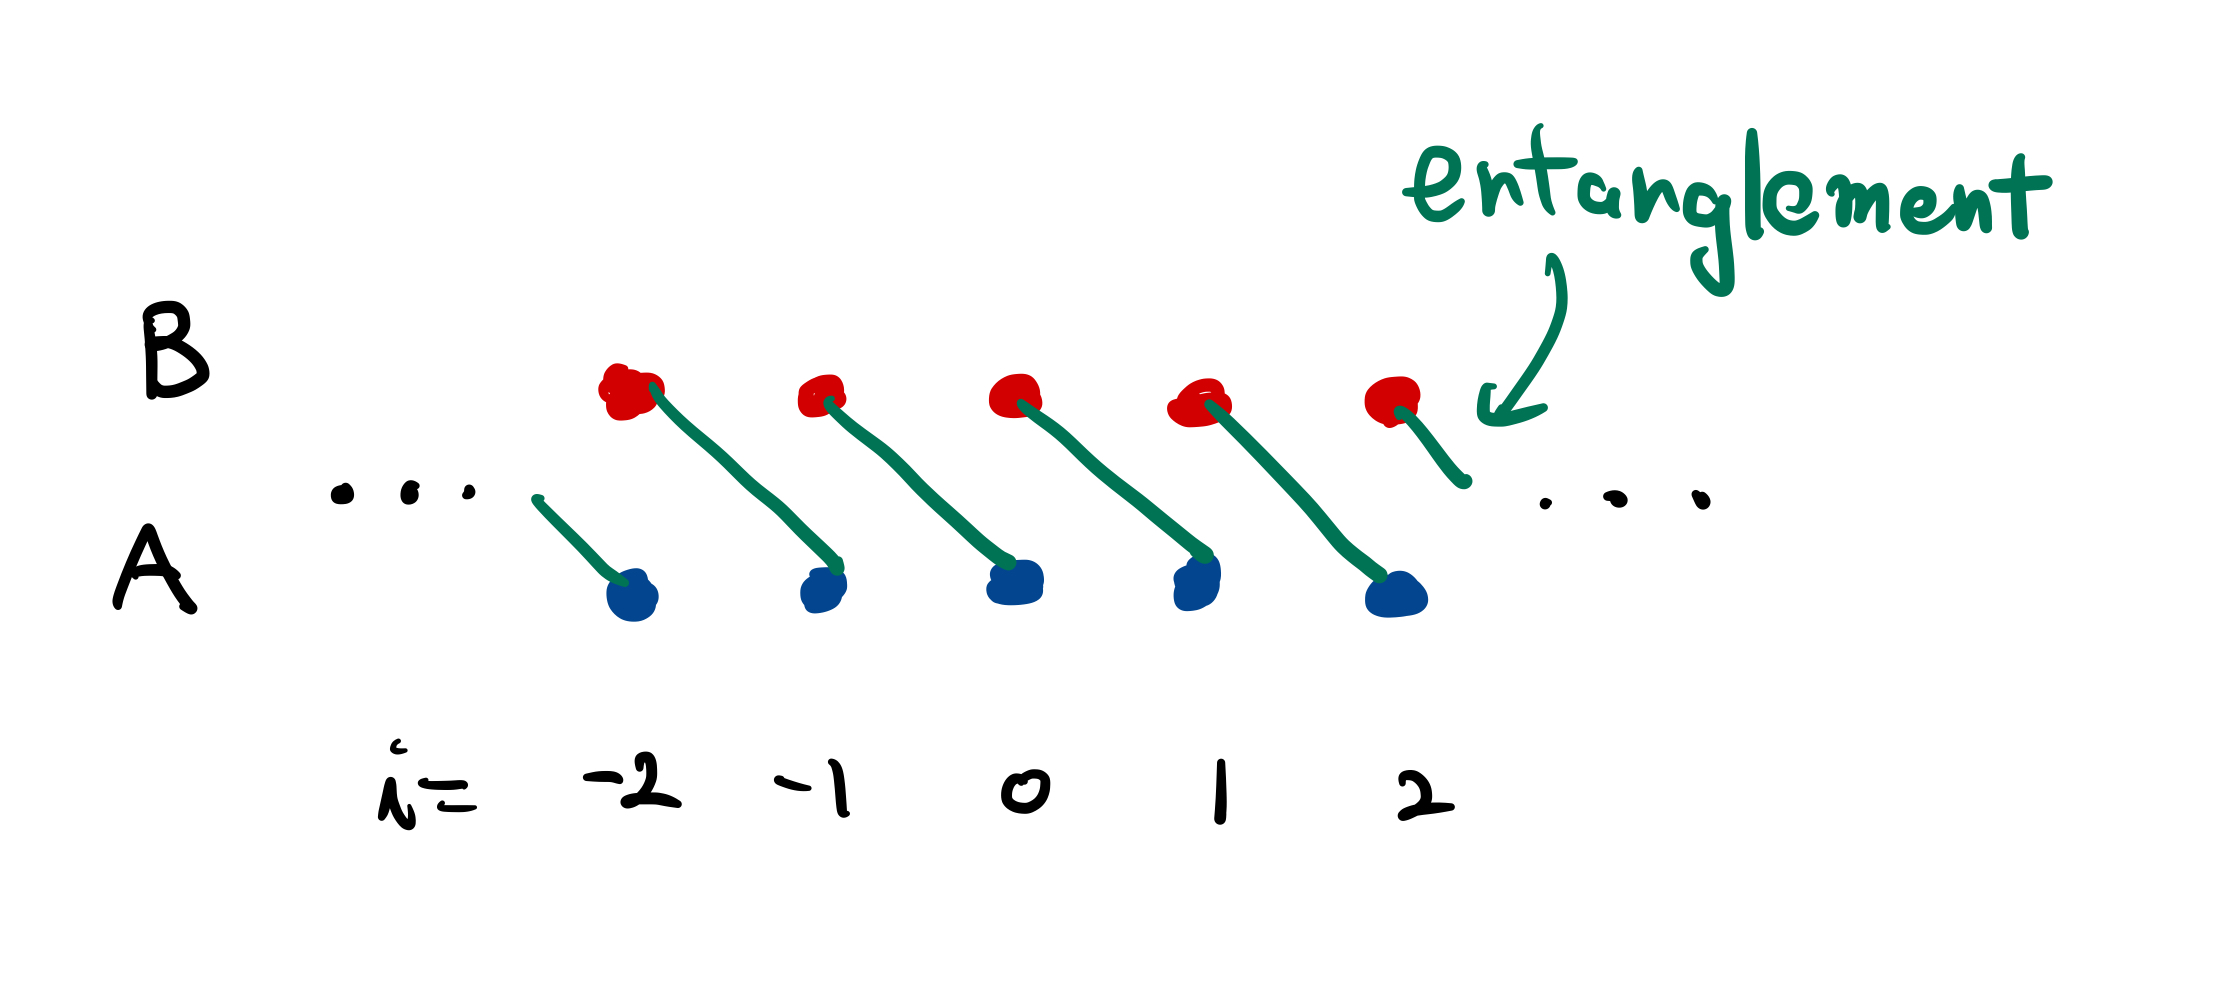
\includegraphics[width=0.5\linewidth]{figs/so3spt} 

}

\caption{The entanglement structure of the state \(\ket{\psi}\) defined in \eqref{eq:SO3SPT}. The \(B\)-qubit at site \(i\) is entangled with the \(A\)-qubit at side \(i+1\), as indicated by the green line.}\label{fig:so3spt}
\end{figure}



We let the group \(SO(3)\) acts on the (projective space of) total states as follows. Let \(T_g^{(i,A)}\) and \(T_g^{(i,B)}\) be the \(SO(3)\) symmetry transformation, defined in Section @ref\{Bloch\}, on the \(A\)- or \(B\)-qubit at the \(i\)-th site. Then the \(SO(3)\) action for which \(\ket{\psi}\) is in SPT is
\begin{equation}
  \label{eq:SO3SPTAction}
  T_g = \prod_{i}T_g^{(i,A)}T_{g^{-1}}^{(i,B)}.
\end{equation}
The state \(\ket{\psi}\) is invariant under this transformation, because \(T_g = \prod_i T_{g^{-1}}^{(i,B)}T_g^{(i+1,A)}\) and \(T_{g^{-1}}^{(i,B)}T_{g}^{(i+1,A)}\) makes the singlet state \(\ket{s_i}\) invariant.
Note that this symmetry transformation does not have the projective phase: it is cancelled between the ones coming from \(U_g^{(i,A)}\) and \(U_{g^{-1}}^{(i,B)}\) within each site.

The direct exposition that \(\ket{\psi}\) is in a SPT can be found in \textcite{Prakash:2018ugo}.
Here instead we observe how the Hypothesis \ref{hyp:SPT} works in this example.
The state \(\ket{\psi}\) has no problem to be defined on a periodic lattice.
However, when there is a boundary, say that only \(i \in \mathbb{Z}_{\ge 0}\) participate in the lattice, the \(A\)-qubit at site \(i=0\) does not have its partner to create an entanglement.
Thus, there are equally good/bad extensions of the state \(\ket{\psi}\) to open boundary:
\begin{equation}
  \label{eq:psiBoundary}
  \ket{\uparrow,\psi} = \ket{\uparrow_{0,A}}\otimes \bigotimes_{i\ge 0}\ket{s_{i}}, \quad
  \ket{\downarrow,\psi} = \ket{\downarrow_{0,A}}\otimes \bigotimes_{i\ge 0}\ket{s_{i}}.
\end{equation}
We call the degrees of freedom \(\ket{\uparrow \! \downarrow_{0,A}}\) the \textbf{edge modes}, as it localizes at the boundary.
On this edge mode, the \(SO(3)\) symmetry acs by \(T_g\), which is exactly the projective representation the qubit has.
This edge mode is \emph{robust} -- if you force the \((i=0,A)\)-qubit be entangled with another qubit (in a finite distance) by some unitary, you get another unentangled qubit, as you cannot erase/create the entanglement by unitaries.
In summary, if we cut the chain in the SPT, on the edge we have the qubit protected by the projective action of \(SO(3)\).

\hypertarget{spt-general-projective-representation}{%
\subsubsection{SPT general projective representation*}\label{spt-general-projective-representation}}

It is easy the generalize the above example into a general projective representation \(R\) of a group \(G\). (Here we assume that \(G\) acts by unitary operations.)
For each site we prepare the local Hilbart space as \(\mathcal{H}_i = R_i \otimes R^\vee_i\), where \(R_i\) is the \(i\)-th copy of \(R\) and \(R^\vee_i\) is the dual of \(R\).
Pick a nonzero state \(\ket{0}\) from \(R\), let \(\ket{0^\vee} \in R^\vee\) denote the dual of \(\ket{0}\), and then define the singlet state \(\ket{s_i}\) by
\begin{equation}
  \label{eq:ketsiGeneral}
  \ket{s_i} = \int \mathrm{d}g \bigl(U_{g^{-1}}\ket{0^\vee}_{(i,B)}\big)\otimes \bigl(U_{g}\ket{0}_{(i+1,A)}\bigr) \in R_{i}^\vee \otimes R_{i+1},
\end{equation}
where \(\mathrm{d}g\) is the Haar measure of \(G\) (it is just a sum over the group element if \(G\) is finite).
This state is invariant under \(T_{g^{-1}}^{(i,B)}T_g^{(i+1,A)}\) (and nonzero).
Now the rest of the constuction is the same as above, and we see the edge mode in \(R\) when the lattice has a boundary.
Thus we have seen how the (one direction of) Hypothesis \ref{hyp:SPT} works in the 1+1d bulk/0+1d boundary case.

\printbibliography

\end{document}
